% --------------------------------------------------------------
% This is all preamble stuff that you don't have to worry about.
% Head down to where it says "Start here"
% --------------------------------------------------------------

\documentclass[10pt]{beamer}

% \usepackage[margin=1in]{geometry}
\usepackage{amsmath,amsthm,amssymb,mathrsfs}
\usepackage{tikz}
\usepackage{wrapfig}
\usepackage{cjhebrew}
% \usepackage[shortlabels]{itemize}

\usepackage[utf8]{inputenc}
\usepackage[english]{babel}

\usetikzlibrary{calc}
\usetikzlibrary{arrows.meta}
\usetikzlibrary{arrows}

\title{Optimal Lipschitz Extension Problem}
\author{Aidan Backus}

\newcommand{\NN}{\mathbb{N}}
\newcommand{\ZZ}{\mathbb{Z}}
\newcommand{\QQ}{\mathbb{Q}}
\newcommand{\RR}{\mathbb{R}}
\newcommand{\CC}{\mathbb{C}}


\newcommand*\dif{\mathop{}\!\mathrm{d}}
\DeclareMathOperator*{\argmin}{argmin}

\DeclareMathOperator{\card}{card}
\DeclareMathOperator{\dist}{dist}
\DeclareMathOperator{\Lip}{Lip}
\DeclareMathOperator{\Lex}{Lex}
\DeclareMathOperator{\hull}{hull}
\DeclareMathOperator{\Stretch}{stretch}
\DeclareMathOperator{\supp}{supp}
\DeclareMathOperator{\Var}{Var}
\DeclareMathOperator{\Exc}{Exc}
\DeclareMathOperator*{\Expect}{\mathbf E}
\newcommand{\normal}{\vec n}
\newcommand{\id}{\mathrm{id}}
\newcommand{\norm}[1]{\left\lVert#1\right\rVert}

\newcommand{\Spec}{\operatorname{Spec}}

\renewcommand{\Re}{\operatorname{Re}}
\renewcommand{\Im}{\operatorname{Im}}

\newtheorem{theoremconjecture}{Theorem-Conjecture}
\newtheorem{conjecture}{Conjecture}
\newtheorem{proposition}{Proposition}
\newtheorem{question}{Question}

\usepackage[backend=bibtex,style=alphabetic,maxcitenames=50,maxnames=50]{biblatex}
\addbibresource{ultrapowerful.bib}
\renewbibmacro{in:}{}
\DeclareFieldFormat{pages}{#1}

\usetheme{AnnArbor}
\usecolortheme{dove}

% \setbeamertemplate{itemize item}{\usebeamerfont*{itemize item}\raise1.25pt\hbox{\donotcoloroutermaths$\bullet$}}
% \setbeamertemplate{itemize subitem}[triangle]
% \setbeamertemplate{itemize subsubitem}[square]

\AtBeginSection{\frame{\sectionpage}}

\begin{document}
% --------------------------------------------------------------
%                         Start here
% --------------------------------------------------------------
\frame{\titlepage}

\section{The Kirszbraun-Valentine theorem}

\begin{frame}{Lipschitz maps}
\begin{definition}
Let $f: X \to Y$ be a mapping between metric spaces and $A \subseteq X$ a set.
The \emph{Lipschitz constant} of $f$ on $A$ is
$$\Lip(f, A) := \sup_{x, y \in A} \frac{\dist_Y(f(x), f(y))}{\dist_X(x, y)}.$$
\end{definition}
 
\begin{problem}
Given a set of Lipschitz mappings $\mathscr F$, find one which is ``optimal''.
\end{problem}
\end{frame}

\begin{frame}{Motivation from Teichm\"uller theory}
\begin{itemize}
\item Let $S$ be a closed surface of Euler characteristic $\chi \leq -2$. 
\begin{itemize}
\item By the Gauss-Bonnet theorem, any Riemannian metric $g$ on $S$ with curvature $K_g$ satisfies 
$$\int_S K_g ~\dif A_g = 2\pi \chi \leq -4\pi,$$
so it is natural to look for $g$ with $K_g = -1$ -- in other words $g$ is \emph{hyperbolic}.
\item There are too many hyperbolic metrics, so we search for a way to understand them en masse. 
\end{itemize}
\item If $g, h$ are hyperbolic metrics, their \emph{Thurston distance} is
$$\dist(g, h) = \inf_{f \sim \id_S} \log \Lip_{(S, g) \to (S, h)}(f, S).$$
\begin{itemize}
\item This metric encodes how geodesics on $(S, g)$ deform when $g$ is deformed (Thurston '86, Papadopoulos '15, Gu\'eritaud and Kassel '17, Daskalopoulos and Uhlenbeck '24...) 
\end{itemize}
\end{itemize}
\end{frame}

\begin{frame}{The Kirszbraun--Valentine theorem}
\begin{itemize}
\item We're going to focus on euclidean space in these lectures.
\begin{itemize}
\item Many of these results extend to Riemannian manifolds, and in particular have applications to understanding deformations of hyperbolic surfaces. 
\end{itemize}
\item First attempt: Find a Lipschitz mapping which minimizes its Lipschitz constant. 
\end{itemize}

\begin{theorem}[Kirszbraun--Valentine theorem]
Let $K$ be a compact subset of $\RR^d$ and $f: K \to \RR^D$ a Lipschitz mapping.
Then there exists $u: \RR^d \to \RR^D$ such that: 
\begin{itemize}
\item $u|_K = f$, 
\item and $\Lip(u, \RR^d) = \Lip(f, K)$.
\end{itemize}
\end{theorem}
\end{frame}

\begin{frame}{Proving the Kirszbraun--Valentine theorem}
\begin{lemma}[Gu\'erituad and Kassel '17]
Let $K$ be a compact subset of $\RR^d$, $f: K \to \RR^D$ a Lipschitz mapping, and $x \notin K$.
For each $\xi \in \RR^D$, let 
$$\varphi(\xi) := \max_{y \in K} \frac{|\xi - f(y)|}{|x - y|}.$$
Then: 
\begin{itemize}
\item There exists a minimum $\xi^*$ of $\varphi$. 
\item Let $K'$ be the set of all $y \in K$ such that $|\xi - f(y)| = \varphi(\xi^*) |x - y|$. Then: 
\begin{itemize}
\item $\xi^* \in \hull(f(K'))$. 
\item There exist $y_1, y_2 \in K'$ such that 
$$\angle(y_1, x, y_2) \leq \angle(f(y_1), \xi^*, f(y_2)),$$
and the latter angle is not zero.
\end{itemize}
\end{itemize}
\end{lemma}
\end{frame}

\begin{frame}{Proving the Kirszbraun--Valentine theorem}
\begin{lemma}[adding points to $K$]
Let $K$ be a compact subset of $\RR^d$, $f: K \to \RR^D$ a Lipschitz mapping, and $x \notin K$.
Then
$$\min_{\xi \in \RR^d} \max_{y \in K} \frac{|\xi - f(y)|}{|x - y|} \leq \Lip(f, K).$$
\end{lemma} 

\begin{itemize}
\item We prove the Kirszbraun--Valentine theorem by iterating this lemma. 
\item Since the only property of euclidean geometry that we used is triangle comparison, this can be made to work in more general metric spaces, subject to constraints on their Alexandrov curvature and a lower bound on $\Lip(f)$.
\end{itemize}
\end{frame}

\begin{frame}{Counterexamples from hyperbolic geometry}
\begin{example}[Gu\'eritaud and Kassel '17]
Let $p$ be a point in the hyperbolic plane $\mathbb H^2$, and draw three geodesics emanating from $p$ which form angles of $2\pi/3$.
Let $K$ be the intersection of these geodesics with a circle centered on $p$.
Define $f(x)$, $x \in K$, to lie on the same geodesic but half the distance from $p$.
Then $\Lip(f) < 1/2$, but any extension of $f$ to $\mathbb H^2$ stretches the geodesics by a factor of $1/2$.
\end{example}

\begin{example}
Let $X$ be a neighborhood of a closed hyperbolic geodesic $\gamma$ and let $f: \partial X \to \mathbb S^1$ be the angle function.
Then any extension of $f$ to $X$ must stretch $\gamma$ more than it does the cycles in $\partial M$.
\end{example}
\end{frame}

\begin{frame}{A failure of uniqueness}
    \centering 
    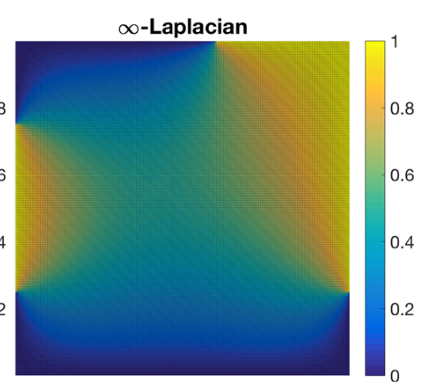
\includegraphics[width=6cm]{KirszbraunValentine.png}
    
\begin{itemize}
\item Adapted from Loisel '20: A minimizing Lipschitz function.  
\item Since the function is nearly constant near the upper-left corner, we can add artificial oscillations there to break uniqueness.
\end{itemize}
\end{frame}

\begin{frame}{Localizing the Lipschitz constant}
\begin{definition}
Let $u: X \to Y$ be a Lipschitz map. Then
$$Lu(x) := \limsup_{r \to \infty} \Lip(u, B(x, r)).$$
\end{definition}

\begin{itemize}
\item The limit superior is actually a limit and an infimum.
\item $Lu$ is upper-semicontinuous, and a proxy for $|\nabla u(x)|_\infty$.
\begin{itemize}
\item Need to take the operator norm $|\cdot|_\infty$ here, not the Frobenius norm $|\cdot|_2$.
\end{itemize}
\item If $X$ is convex then 
$$\Lip(u, X) = \sup_{x \in X} Lu(x).$$
\end{itemize}
\end{frame}

\begin{frame}{A much bigger failure of uniqueness}

\begin{theorem}[B, Ze-An '24: solving the eikonal equation]
Let $\Gamma$ be a closed subset of $\RR^d$, $f: \RR^d \to \RR^D$ a Lipschitz map, and $\psi$ a continuous function on $\RR^d \setminus \Gamma$.
If $\psi \geq Lf$ then there exists $u: \RR^d \to \RR^D$ such that $Lu = \psi$ on $\RR^d \setminus \Gamma$ and $u = f$ on $\Gamma$.
\end{theorem}

\begin{lemma}[creating oscillations without destructive interference]
Let $u_0 := f$ and $\mathscr L_0 := \emptyset$.
Then for each $i \in \NN$ there is a set of line segments $\mathscr L_i$, which are evenly spaced at scale $2^{-i}$, and a map $u_i$, such that:
\begin{itemize}
\item For each $\ell \in \mathscr L_i$ and $x \in \ell$, $\Lip(u_i, \ell) > \psi(x) - 2^{-i}$.
\item $u_i = u_{i - 1}$ on a $2^{-i}$-neighborhood of $\Gamma \cup \bigcup_{j < i} \mathscr L_j$.
\end{itemize}
\end{lemma}

\begin{problem}
Which functions can be $Lu$ for a Lipschitz map $u$?
\end{problem}
    
\end{frame}

%%%%%%%%%%%%%%%%%%%%%%%%%%%%
\section{The \texorpdfstring{$\infty$-Laplacian}{infinity-Laplacian}}

\begin{frame}{Absolutely minimizing Lipschitz mappings}
\begin{itemize}
\item The problem is that variational problems defined by integrals already locally minimize, but not $L^\infty$ variational problems. 
\item Second attempt: Try a more localized version of the Lipschitz minimization property. 
\end{itemize}

\begin{definition}
A mapping $u: X \to Y$ is \emph{absolutely minimizing Lipschitz} (\emph{AML}) if there is a basis $\mathscr U$ of open subsets of $X$ such that
\begin{itemize}
\item for every basic open set $U \in \mathscr U$,
\item and every $v: U \to Y$ with $\Lip(v, \partial U) = \Lip(u, \partial U)$, 
\end{itemize}
one has
$$\Lip(u, U) \leq \Lip(v, U).$$
\end{definition}
\end{frame}

\begin{frame}{Well-posedness of AML scalar fields}
\begin{itemize}
\item In general, AML mappings are too hard, but AML scalar fields are easier. 
\item Recall the $p$-Laplacian 
$$\Delta_p u := \nabla \cdot (|\nabla u|^{p - 2} \nabla u) = 0$$
whose solutions minimize $\|\nabla u\|_{L^p}$. 
\item Aronsson '67: Since $\|\nabla u\|_{L^p} \to \Lip(u, U)$ as $p \to \infty$, study $p$-harmonic functions as $p \to \infty$. 
\end{itemize}

\begin{theorem}[Jensen '93: wellposedness of AML functions]
Let $U \subseteq \RR^d$ be an open set with Lipschitz boundary, and $f: \partial U \to \RR$ a Lipschitz function. Then: 
\begin{itemize}
\item There is a unique AML function $u: U \to \RR$ such that $u|_{\partial U} = f$. 
\item Let $u_p$ be the unique $p$-harmonic extension of $f$.
Then $u_p \to u$ in $C^0$ as $p \to \infty$.
\end{itemize}
\end{theorem}
\end{frame}

\begin{frame}{The $\infty$-Laplacian}
\begin{itemize}
\item The $p$-Laplacian is quasilinear and its solutions are only $C^{1 + \alpha}$.
\begin{itemize}
\item In Aronsson's time, the $p$-Laplacian could only be understood in divergence form: for every $\chi \in C^\infty_c(U)$,
$$(\nabla \chi, |\nabla u|^{p - 2} \nabla u)_{L^2(U)} = 0.$$
\end{itemize}
\item Pretend for a moment that we could legally write the $p$-Laplacian in nondivergence form 
$$(p - 2) |\nabla u|^{p - 4} \langle \nabla^2 u, \nabla u \otimes \nabla u\rangle + |\nabla u|^{p - 2} \Delta u = 0.$$
Renormalize and take $p \to \infty$ to find the limiting PDE: 
\end{itemize} 

\begin{definition}
The \emph{$\infty$-Laplacian} is the PDE 
$$\Delta_\infty u := \langle \nabla^2 u, \nabla u \otimes \nabla u\rangle = 0.$$
\end{definition}
\end{frame}

\begin{frame}{Classical solutions of the $\infty$-Laplacian}
\begin{itemize}
\item Affine functions.
\item $|x|$, on the punctured space.
\item $x_1^{4/3} - x_2^{4/3}$, on Quadrant I.
\item $\arctan(x_2/x_1)$, on the Riemann surface of $\log$.
\item Classical solutions of the eikonal equation $|\nabla u| = \lambda$.
\end{itemize}
\end{frame}

\begin{frame}{The $\infty$-Laplacian is a horrible PDE}
\begin{itemize}
\item $\Delta_\infty$ is totally nonlinear, and only elliptic in the $\nabla u$ direction.  
\begin{itemize}
\item So $u$ should not have much more regularity than Lipschitz. 
\item $x^{4/3} - y^{4/3}$ is AML, but is only $C^{1 + 1/3}$. 
\item According to Evans and Smart '11, in $d = 2$ you should think of $\Delta_\infty$ as a totally nonlinear parabolic PDE where the time vector field is $\nabla^2 u \cdot \nabla u$ and the space vector field is $\nabla u$. 
\end{itemize}
\item We cannot define solutions using integration by parts. 
\begin{itemize}
\item $\Delta_\infty$ cannot be written in divergence form. 
\item So Aronsson got stuck here.
\end{itemize}
\end{itemize}
\end{frame}

\begin{frame}{The miracle on the viscosity-ula}
\begin{itemize}
\item The correct solution concept was introduced by Crandall, Evans, and Lions '84 in their work on Hamilton-Jacobi equations. 
\item Too hard to motivate for the $\infty$-Laplacian a priori, so let's do it for inviscid Burgers' equation first:
$$\partial_t u + u \partial_x u = 0.$$
This has way too many solutions!  
\item The physically correct solutions are $C^0$ limits of the viscous problem 
$$\partial_t u + u \partial_x u = \varepsilon \partial_x^2 u.$$
This is a semilinear parabolic PDE, so it satisfies the maximum principle: 
\begin{itemize}
\item If $v \in C^2$ and $u - v$ has a local maximum at $(x_*, t_*)$, then
$$\partial_t v(x_*, t_*) + v(x_*, t_*) \partial_x v(x_*, t_*) \leq \varepsilon \partial_x^2 v(x_*, t_*).$$
\end{itemize}
\end{itemize}
\end{frame}

\begin{frame}{Viscosity solutions of inviscid Burgers}
\begin{itemize}
\item The maximum principle is a result about pointwise comparison, so it's preserved by $C^0$ limits. 
\item So, if $u$ is a solution of inviscid Burgers which is physically meaningful, it is a viscosity solution: 
\end{itemize}

\begin{definition}
Let $u \in C^0((-T, T) \times \RR)$. We say that $u$ is a \emph{viscosity solution of inviscid Burgers' equation} if, for every $v \in C^1((-T, T) \times \RR)$:  
\begin{itemize}
\item If $u - v$ has a local maximum at $(x_*, t_*)$, then
$$\partial_t v(x_*, t_*) + v(x_*, t_*) \partial_x v(x_*, t_*) \leq 0.$$
\item If $u - v$ has a local minimum at $(x_*, t_*)$, then 
$$\partial_t v(x_*, t_*) + v(x_*, t_*) \partial_x v(x_*, t_*) \geq 0.$$
\end{itemize}
\end{definition}
\end{frame}

\begin{frame}{Viscosity solutions of the $\infty$-Laplacian}
\begin{lemma}[maximum principle for the $p$-Laplacian]
Suppose that $U$ is an open set with Lipschitz boundary, $\Delta_p u \geq 0$, and $\Delta_p v \leq 0$, and $u \leq v$ on $\partial U$.
Then $u \leq v$ on $U$.
\end{lemma}   
 
\begin{definition}
Let $u \in C^0(U)$. Then:
\begin{itemize}
\item $u$ is \emph{$\infty$-subharmonic} at $x_* \in U$ (or that $\Delta_\infty u \geq 0$ \emph{in the sense of vanishing viscosity}), if, for every $v \in C^2(U)$ such that $u - v$ has a local maximum at $x_*$,
$$\Delta_\infty v(x_*) \geq 0.$$
\item $u$ is \emph{$\infty$-superharmonic} if $-u$ is $\infty$-subharmonic.
\item $u$ is \emph{$\infty$-harmonic} if $u$ is $\infty$-subharmonic and $\infty$-superharmonic.
\end{itemize}
\end{definition}
\end{frame}

\begin{frame}{Existence} 
\begin{proposition}[solving the $\infty$-Laplacian]
Let $U \subset \RR^d$ have a Lipschitz boundary and finite volume, and let $f$ be a Lipschitz function on $\partial U$.
Then there is an $\infty$-harmonic extension $u$ of $f$. Moreover,
$$\Lip(u, U) = \Lip(f, \partial U).$$
\end{proposition}

\begin{lemma}[$W^{1, r}$ estimate on the $p$-Laplacian]
Let $U \subset \RR^d$ have a Lipschitz boundary, and let $f$ be a Lipschitz function on $\partial U$.
Let $1 < r \leq p < \infty$, and let $u_p$ be the $p$-harmonic extension of $f$. Then
$$\|\nabla u_p\|_{L^r} \leq \operatorname{vol}(U)^{1/r} \Lip(f, \partial U) .$$
\end{lemma}
\end{frame}

%%%%%%%%%%%%%%%%%%%%%
\section{Properties of \texorpdfstring{$\infty$-harmonic}{infinity-harmonic} functions}

\begin{frame}{Uniqueness}
\begin{theorem}[Jensen's maximum principle]
Suppose that $u$ is $\infty$-subharmonic and $v$ is $\infty$-superharmonic on $U$.
If $u \leq v$ on $\partial U$, then $u \leq v$.
\end{theorem}

\begin{lemma}
Jensen's maximum principle holds if we additionally assume that there exists $\kappa > 0$ such that $\Delta_\infty u \geq \kappa$.
\end{lemma}

\begin{lemma}
Suppose that $u$ is $\infty$-subharmonic on $U$, and $\varepsilon > 0$.
Then there is an $\infty$-subharmonic function $u_\varepsilon$, such that: 
\begin{itemize}
\item $u_\varepsilon = u$ on $\{|\nabla u| \geq \varepsilon\} \cup \partial U$, but  
\item on $\{|\nabla u| < \varepsilon\}$, $u_\varepsilon$ is a viscosity solution of $|\nabla u_\varepsilon| = \varepsilon$.
\end{itemize}
\end{lemma}
\end{frame}

\begin{frame}{Regularity}
\begin{theorem}
Let $u$ be $\infty$-harmonic. Then: 
\begin{itemize}
\item (Evans and Savin '08) If $d = 2$, then for some $\alpha > 0$, $u \in C^{1 + \alpha}$. 
\item (Evans and Smart '11) $u$ is differentiable. 
\end{itemize}
\end{theorem}

\begin{problem}
    What is the sharp regularity of $\infty$-harmonic functions?
\end{problem}

\begin{problem}
    Let $u$ be a $C^2$ $\infty$-harmonic function on a domain in $\RR^2$, such that $|\nabla^2 u \nabla u| \geq \varepsilon$.
    If $v$ is an $\infty$-harmonic function and a small perturbation of $u$, can we get higher regularity for $v$?
\end{problem}
\end{frame}

\begin{frame}{Comparison with cones}

\begin{itemize}
\item By Jensen's maximum principle applied to the punctured ball, if $u$ is $\infty$-subharmonic, $u(0) = 0$, and $|x| = r$ implies $u(x) \leq |x|$, then $|x| \leq r$ implies $u(x) \leq |x|$. 
\end{itemize}

\begin{definition}
A function $u \in C^0(U)$ satisfies: 
\begin{itemize}
\item \emph{comparison with cones from above}, if for every $B(x_*, r) \Subset U$, if $u(x) \leq u(x_*) + B|x - x_*|$ for $x \in \partial B(x_*, r)$, then the same inequality holds for $x \in B(x_*, r)$.
\item \emph{comparison with cones}, if $u$ and $-u$ both satisfy comparison with cones from above. 
\end{itemize}
\end{definition}

\begin{proposition}
A function $u \in C^0(U)$ is $\infty$-subharmonic iff $u$ satisfies comparison with cones from above.
\end{proposition}
\end{frame}

\begin{frame}{Characterization of $\infty$-harmonic functions}
\begin{theorem}
Let $U \subseteq \RR^d$ be a bounded Lipschitz domain.
The following are equivalent for $u \in C^0(U)$: 
\begin{enumerate}
\item $u$ is $\infty$-harmonic. 
\item $u$ satisfies comparison with cones. 
\item $u$ is absolutely minimizing Lipschitz. 
\item $u$ is the limit in $C^0$ of $p$-harmonic functions as $p \to \infty$. 
\item $u$ is the limit in $C^0$ of values of tug-of-war games at scale $\varepsilon$, as $\varepsilon \to 0$. 
\end{enumerate}
\end{theorem}
    
\begin{itemize}
    \item We showed that 1, 2, and 4 are equivalent. 
    \item Let us show that 2 is equivalent to 3. 
    \item Time permitting, we will define 5 and sketch that 3 is equivalent to 5.
\end{itemize}
\end{frame}

\begin{frame}{Tug of war}
\begin{itemize}
\item Let $(X, E)$ be an (undirected, unweighted, possibly infinite) graph and $Y \subset X$. 
\item Introduce \emph{Alice's payoff for tug-of-war} $f: Y \to \RR$.  
\begin{itemize}
\item Alice and Bob are going to play a game where the set of game states is $X$, and the set of terminal game states is $Y$.
\item If the final game state is $y \in Y$, Bob will pay Alice $f(y)$.  
\end{itemize}
\item Suppose that the game is in state $x \in X$.  
\begin{itemize}
\item Alice flips a coin.
\item If it's heads, it's Alice's turn. Otherwise it's Bob's turn.
\item The player whose turn it is moves the game to a state $x'$ adjacent to $x$.
\item If $x' \in Y$, the game ends.
\end{itemize}
\end{itemize}
\end{frame}

\begin{frame}{Strategies}
\begin{itemize}
\item A \emph{strategy for tug-of-war} is a mapping which sends $x \in X$ to a probability distribution on the set of vertices adjacent to $x$. 
\begin{itemize} 
\item Suppose that Alice's strategy is $S$, the game is in state $x$, and Alice won the coin toss. 
\item Then Alice uses the probability distribution $S(x)$ to draw a vertex $x'$ adjacent to $x$ at random.
\item Alice then moves the game state to $x'$. 
\end{itemize}
\item \emph{Alice's value function for tug-of-war} $u(x)$ at $x \in X$ is
\begin{itemize}
\item the supremum over all strategies $S_{\rm Alice}$
\item of the infimum over all strategies $S_{\rm Bob}$
\item of the expected value of Alice's payoff $f(y)$, where $y$ is the end state of the game such that:
\begin{itemize}
\item the initial state of the game was $x$, and
\item Alice and Bob played the strategies $S_{\rm Alice}$ and $S_{\rm Bob}$.
\end{itemize}
\end{itemize}
\end{itemize}
\end{frame}

\begin{frame}{Dynamic programming}
\begin{itemize}
\item Alice's optimal strategy is to always move in a direction which increases her value function as much as possible. 
\item However, she only has a half-chance to move, and otherwise (if he is playing optimally) Bob will decrease Alice's value function as much as possible.  
\end{itemize}

\begin{proposition}
Let $u$ be Alice's value function for tug-of-war. Then 
$$u(x) = \frac{1}{2} \left[\sup_{x_{\rm Alice} \sim x} u(x_{\rm Alice}) + \inf_{x_{\rm Bob} \sim x} u(x_{\rm Bob})\right].$$
\end{proposition}  

\begin{itemize}
\item The finite difference equation for $u$ looks suspiciously like the $\infty$-Laplacian... 
\end{itemize}
\end{frame}

\begin{frame}{Tug-of-war at scale $\varepsilon$}
\begin{definition}
Let $X$ be a metric space, $Y \subset X$, $\varepsilon > 0$, and $\{x, x'\} \in E$ iff $\dist(x, x') < \varepsilon$.
Then \emph{tug-of-war at scale $\varepsilon$} on $X$ is the game just described with the graph $(X, E)$ and set of final states $Y$.
\end{definition} 

\begin{theorem}[Peres, Schramm, Sheffield, and Wilson '08]
Suppose that $X$ is a length space and $Y \subset X$ is nonempty.
Let $f: Y \to \RR$ be bounded Lipschitz function with a uniformly continuous extension to $X$.
Then: 
\begin{itemize}
\item Let $f$ be Alice's payoff for a game of tug-of-war at scale $\varepsilon$.
Then Alice's value function $u_\varepsilon$ is well-defined and uniformly continuous on $X$.
\item There exists an AML function $u$ such that $\|u - u_\varepsilon\|_{C^0} \lesssim \varepsilon$. 
\end{itemize}
\end{theorem}
\end{frame}

%%%%%%%%%%%%%%%%%%%%%
\section{The stretch set of a \texorpdfstring{$\infty$-harmonic}{infinity-harmonic} function}

\begin{frame}{Stretch sets}
\begin{definition}[Thurston '86]
Let $u: X \to Y$ be a Lipschitz map and $U \subseteq X$ an open set. The \emph{stretch set} of $u$ on $U$ is 
$$\Stretch(u, U) := \{x \in U: Lu(x) = \Lip(u, U)\}.$$
\end{definition}

\begin{itemize}
\item Clearly a relatively closed subset of $U$.
\item Our next task is to understand the geometry of $\Stretch(u, U)$.
\end{itemize}
    
\end{frame}

\begin{frame}{Geodesic laminations}
\begin{definition}
A \emph{geodesic lamination} is a closed set $\lambda \subseteq U$ equipped with a partition of $\lambda$ into line segments $\gamma$, called \emph{leaves}, such that $\partial \gamma \subseteq \partial U$. 
\end{definition}

\begin{itemize}
\item Mainly studied in hyperbolic surfaces. A picture from Thurston '97 in that case:
\end{itemize}

\centering 
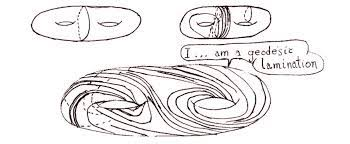
\includegraphics[width=7cm]{GeodesicLamination.jpg}
    
\end{frame}

\begin{frame}{Transverse measures}
\begin{itemize}
\item If $\lambda$ is a geodesic lamination, then we can cover $U$ by open sets $V$ such that the space of leaves of $\lambda \cap V$ is a locally compact metrizable space, which we call the \emph{local leaf space} in $V$.
\item A \emph{$d - 1$-current of locally finite mass} on $U$ is a continuous linear functional on the space of compactly supported continuous $1$-forms on $U$.
\end{itemize}

\begin{definition}
Let $\lambda$ be a geodesic lamination.
A \emph{transverse measure} $T$ to $\lambda$ is a nonzero $d - 1$-current of locally finite mass, such that:
\begin{itemize}
\item for each open set $V$ with a local leaf space $K_V$, there is a positive Radon measure $\mu_V$ on $K_V$, such that:
\item for each continuous $1$-form $\varphi$ with compact support in $V$,
$$\langle T, \varphi\rangle = \int_{K_V} \left[\int_\gamma \varphi\right] \dif \mu_V(\gamma).$$
\end{itemize}
\end{definition}
\end{frame}

\begin{frame}{The geodesic lamination in the stretch set}
\begin{theorem}[Daskalopoulos and Uhlenbeck '20]
Let $u$ be an $\infty$-harmonic function on $U$ such that $\Stretch(u, U)$ is nonempty.
Then $\Stretch(u, U)$ is a geodesic lamination, and for any leaf $\gamma \subseteq \Stretch(u, U)$,
$$\frac{\dif}{\dif t} u(\gamma(t)) = \Lip(u, U).$$
\end{theorem}

\begin{lemma}[leaves are straight lines]
Let $x \in \Stretch(u, U)$.
If $B(x, r) \Subset U$, then there exists $x_+, x_- \in \partial B(x, r)$ such that:
\begin{itemize}
\item $[x, x_+], [x, x_-] \subseteq \Stretch(u, U)$.
\item $u(x_\pm) = u(x) \pm \Lip(u, U)r$.
\end{itemize}
\end{lemma}

\begin{lemma}[leaves are disjoint]
Two maximal line segments in $\Stretch(u, U)$ must be disjoint.
\end{lemma}
\end{frame}

\begin{frame}{Dualizing the $p$-Laplacian}
\begin{itemize}
\item Suppose that $d = 2$. Suppose that $u$ is $p$-harmonic:
$$\nabla \cdot (|\nabla u|^{p - 2} \nabla u) = 0.$$
\item We can rewrite this as
$$\nabla \times (|\nabla u|^{p - 2} \nabla^\perp u) = 0,$$
so there exists $v$ such that
$$\nabla v = |\nabla u|^{p - 2} \nabla^\perp u.$$
\item By H\"older-chasing, if $1/p + 1/q = 1$ then $v$ is $q$-harmonic!
\end{itemize}
\end{frame}

\begin{frame}{The dual problem}
\begin{definition}
A $BV$ function $v$ on $U$ has \emph{least gradient}, if (among all functions with the same trace), $v$ minimizes its total variation
$$\int_M |\nabla v| \dif V.$$
\end{definition}

\begin{theorem}[Daskalopoulos and Uhlenbeck '20]
Suppose that $d = 2$, and $u_p$ are $p$-harmonic functions on $U$ converging to an $\infty$-harmonic function $u$, which is normalized so that $\Lip(u, U) = 1$.
Let $v_q$ be the dual $q$-harmonic harmonic to $u_p$.
Then:
\begin{itemize}
\item $v_q$ converges in the weakstar topology of $BV$ to a function $v$ of least gradient.
\item If $v$ is not constant, then $\nabla v$ is a transverse measure to $\Stretch(u, U)$.
\end{itemize}
\end{theorem}
\end{frame}

\begin{frame}{Constructing the transverse measure}
\begin{itemize}
\item We renormalize by replacing $v_q$ with $k_p^{p - 1} v_q$ where $k_p^{1 - p} := \|\nabla u_p\|_{L^p}^p$ (so $k_p \to 1$).
\end{itemize}

\begin{lemma}[B '24]
$$\frac{1}{q} \int_U |\nabla v_q|^q \dif V + \frac{k_p^p}{p} \int_U |\nabla u_p|^p \dif V = k_p \int_U \nabla u_p \cdot \nabla v_q \dif V.$$
\end{lemma}

\begin{itemize}
\item Total variation is lower-semicontinuous in the weakstar topology of $BV$, so by compensated compactness,
$$\int_U |\nabla v| \dif V \leq \int_U \nabla u \cdot \nabla v \dif V \leq \int_U |\dif v| \dif V.$$
\item Since $|\dif v| \dif V$ is a positive Radon measure, this forces $|\nabla v| = \nabla u \cdot \nabla v$ as Radon measures, so 
\begin{itemize}
\item it is necessary that $v$ have least gradient and $\nabla v$ be transverse.
\end{itemize}
\end{itemize}
\end{frame}

\begin{frame}{Possible applications of the duality}
\begin{itemize}
\item Next few slides are very speculative!
\item A slight generalization of the above proof yields:
\end{itemize}

\begin{theorem}
Let $T$ be a mass-minimizing $d - 1$-current.
Then there exists a geodesic lamination $\lambda$ such that $T$ is transverse to $\lambda$.
\end{theorem}

\begin{itemize}
\item When $d = 2$, the fact that least gradient functions give a geodesic lamination leads to an equivalence between the least gradient problem and the Monge--Kantorovich problem in optimal transport.
\begin{itemize}
\item G\'orny '21: Applications of optimal transport to the regularity theory of the $1$-Laplacian when $d = 2$.
\end{itemize}
\end{itemize}

\begin{problem}
Do the theorems of G\'orny '21 also hold for mass-minimizing $d - 1$-currents?
\end{problem}
\end{frame}

\begin{frame}{More possible applications}
    
\begin{itemize}
\item As we will later see, defining the $\infty$-Laplacian on vector-valued or manifold-valued maps seems impossibly hard.
\begin{itemize}
\item Maz\'on, Rossi, and Segura de L\'eon '14 and G\'orny and Maz\'on '21 \emph{defined} weak solutions of $BV$ variational problems in terms of the duality with $L^\infty$ variational problems.
\end{itemize}
\item A generalization of the $\infty$-Laplacian to vector-valued maps could perhaps be based on a resolution of:
\end{itemize}

\begin{problem}
Formulate the $\infty$-Laplacian purely in terms of its duality with the $1$-Laplacian.
\end{problem}

\begin{example}
Let $U$ be a disk in the right half-plane centered on the $x$-axis, and let $u(x, y) := \arctan(y/x)$.
Then $\Stretch(u, U)$ is empty, so the dual $1$-harmonic function is $0$.
\end{example}
    
\begin{itemize}
\item No idea how to overcome this.
\end{itemize}

\end{frame}

\begin{frame}{Two problems posed by Daskalopoulos and Uhlenbeck}
\begin{problem}
Verify that the theory of $\infty$-harmonic functions, in particular the theorems of Evans and Savin, and Evans and Smart, goes through unchanged on a (simply connected) Riemannian manifold (and more generally, for scalar-valued $L^\infty$ variational problems).
\end{problem}

\begin{problem}
Let $M$ be a closed oriented Riemannian manifold, and let $\rho$ be a homotopy class of maps from $M$ to the circle.
Show that there is a unique $\infty$-harmonic map representing $\rho$.
\end{problem}
\end{frame}

\section{AML maps between manifolds}
\begin{frame}{Existence and uniqueness}
\begin{problem}
Let $U$ be a Lipschitz domain in $\RR^d$ and $f: \partial U \to \RR^D$ a Lipschitz map.
Does there exist an AML extension of $f$ to $U$?
\end{problem}

\begin{example}[Sheffield and Smart '10]
On the unit disk, for each $t \in [0, 1]$, let
$$u_t(re^{i\theta}) := tr^2e^{2i\theta} + (1 - t) re^{2i\theta}.$$
Then $u_t(e^{i\theta}) = e^{2i\theta}$ (independently of $t$) but $u_t$ is AML.
So uniqueness fails quite badly.
\end{example}
\end{frame}

\begin{frame}{A toy problem on graphs}
\begin{itemize}
    \item Idea (Sheffield and Smart '10): Look for an even stronger condition than AML, to try to get uniqueness.
    \item Do a toy problem on finite graphs $(X, E)$ first, with a set of ``boundary'' vertices $Y \subset X$.
\end{itemize}

\begin{definition}
Let $u: X \to \RR^D$. For $x \in X$, consider the \emph{local Lipschitz constant}
$$Su(x) := \max_{y \sim x} |u(y) - u(x)|.$$
Say that $u \preceq v$ if $u|_Y = v|_Y$ and
$$\max_{Su > Sv} Su \leq \max_{Sv > Su} Sv.$$
\end{definition}
\end{frame}

\begin{frame}{Well-posedness of the toy problem}
\begin{definition}
A map $u: X \to \RR^D$ is \emph{tight} if $u$ is $\preceq$-minimal.
\end{definition}

\begin{lemma}
Let $\Lex(u) \in \RR^{\card X}_+$ be the list of values of $Su$, sorted to be nonincreasing.
If
\begin{itemize}
\item for every $v$ such that $u|_Y = v|_Y$, $\Lex(u)$ is lexicographically prior to $\Lex(v)$,
\end{itemize}
then $u$ is tight.
\end{lemma}

\begin{theorem}[well-posedness of discrete tight maps]
Given $f: Y \to \RR^D$ there is a unique tight extension of $f$ to $X$.
\end{theorem}

\begin{itemize}
    \item For existence, we use the lemma and induction on $\card X$.
    \item Let's skip the proof of uniqueness.
\end{itemize}
\end{frame}

\begin{frame}{Going to the continuum}
\begin{definition}[Sheffield and Smart '10]
Let $U \subseteq \RR^d$ be an open set, and $u, v: U \to \RR^D$.
We say that $u \preceq v$ if $u|_{\partial U} = v|_{\partial U}$ and
$$\sup_{Lu > Lv} Lu \leq \sup_{Lv > Lu} Lv.$$
If $u$ is $\preceq$-minimal, then $u$ is \emph{tight}.
\end{definition}

\begin{lemma}
If $u$ is tight, then $u$ is AML.
\end{lemma}

\begin{itemize}
\item To get minimality on an open set $V$, compare to $v$ which agrees with $u$ on $U \setminus V$ and is given by the Kirszbraun-Valentine theorem on $V$.
\end{itemize}

\begin{problem}
Given $f: \partial U \to \RR^D$ Lipschitz, does there exist a unique tight extension of $f$ to $U$?
\end{problem}
\end{frame}

\begin{frame}{The Schatten norms}
\begin{definition}
Let $\mathcal H_1, \mathcal H_2$ be Hilbert spaces, and $A: \mathcal H_1 \to \mathcal H_2$ a bounded linear map.
\begin{itemize}
\item The \emph{positive-semidefinite part} of $A$ is
$$Q(A) := \sqrt{AA^\dagger} \in \mathcal B(\mathcal H_2).$$
\item For $p \in [1, \infty]$, the $p$th \emph{Schatten norm} of $A$, $|A|_p$, is the $\ell^p$ norm of the eigenvalues of $Q(A)$.
\item A unit vector $\xi \in \mathcal H_1$ is a \emph{top singular vector} of $A$, if $|A\xi| = |A|_\infty$.
\end{itemize}
\end{definition}

\begin{itemize}
\item So $|A|_2$ is the Frobenius norm, and $|A|_\infty$ is the operator norm.
\item Our instinct is to use the Frobenius norm with $\nabla u$, but...
\end{itemize}

\begin{lemma}
Let $u$ be a smooth map. Then $Lu(x) = |\nabla u(x)|_\infty$.
\end{lemma}

\end{frame}

\begin{frame}{A PDE for smooth tight maps}
\begin{theorem}[Sheffield and Smart '10: Euler-Lagrange equation]
Let $u: U \to \RR^D$ be a smooth mapping such that
\begin{itemize}
\item There exists a unit vector field $\xi$, such that for each $x \in U$, $\xi(x)$ is the unique top singular vector of $\nabla u(x)$.
\end{itemize}
Then $u$ is tight iff 
$$\langle \nabla \langle \nabla u, \xi\rangle, \xi\rangle = 0.$$
\end{theorem}

\begin{itemize}
\item Reduces to the $\infty$-Laplacian when $D = 1$ (take $\xi = \nabla u/|\nabla u|$).
\item Doesn't make sense if $u$ is conformal... like if $u$ is the identity.
\end{itemize}
\end{frame}

\begin{frame}{Proof of the PDE characterization}
\begin{lemma}
Let $A$ be a linear map, and let $\xi$ be the unique top singular vector of $A$. Then
$$|A + \varepsilon B|_\infty^2 = |A|_\infty^2 + 2\varepsilon \langle A\xi, B\xi\rangle + O(\varepsilon^2)$$
where the implied constant only depends on $|A|_\infty$, $|B|_\infty$, and the difference between the first two singular values of $A$.
\end{lemma}

\begin{lemma}
If $u$ is a smooth tight map, and $\xi$ is as in the theorem, then $u$ pushes forward every integral curve of $\xi$ to a straight line.
\end{lemma}
\end{frame}

\begin{frame}{Another attempt: bringing back the $p$-Laplacian}
\begin{itemize}
\item Problems with tightness:
\begin{itemize}
\item Well-posedness seems like a nightmare to prove: more on that later.
\item No PDE for conformal maps.
\item Not clear what its relation with $L^p$ or $BV$ problems is.
\end{itemize}
\item What if we declared by fiat that the AML map should arise from the $p$-Laplacian?
\begin{itemize}
\item Then existence would be easy to prove.
\end{itemize}
\end{itemize}

\begin{definition}[Daskalopoulos and Uhlenbeck '22]
Let $1 < p < \infty$.
A $W^{1, p}$ map $u$ is \emph{(Schatten) $p$-harmonic} if
$$\nabla \cdot (Q(\nabla u)^{p - 2} \nabla u) = 0.$$
\end{definition}
\end{frame}

\begin{frame}{Properties of $p$-harmonic maps}
\begin{lemma}[Euler-Lagrange equation]
Let $u \in W^{1, p}$. Then $u$ is $p$-harmonic iff $u$ minimizes $\||\nabla u|_p\|_{L^p}$.
\end{lemma}

\begin{lemma}[well-posedness and $W^{1, r}$ estimate for Schatten $p$-Laplacian]
Given a Lipschitz map $f$ on $\partial U$, there is a unique $p$-harmonic extension $u$ of $f$ to $U$.
Moreover, if $r \leq p$ then
$$\||\nabla u|_r\|_{L^r} \leq (d\mathrm{vol}(U))^{1/r} \Lip(f, \partial U).$$
\end{lemma}
    
\end{frame}

\begin{frame}{Existence and geodesic lamination}
    
\begin{definition}[Daskalopoulos and Uhlenbeck '22]
A map $u$ is \emph{(Schatten) $\infty$-harmonic} if there exist Schatten $p$-harmonic maps $u_p$ such that for every $1 < r < \infty$, $u_p \rightharpoonup u$ in $W^{1, r}$.
\end{definition}

\begin{proposition}[solving the Schatten $\infty$-Laplacian]
    Given a Lipschitz map $f$ on $\partial U$, there is an $\infty$-harmonic extension $u$ of $f$ to $U$.
    Moreover,
    $$\Lip(u, U) = \Lip(f, \partial U).$$
\end{proposition}

\begin{itemize}
    \item For $\infty$-harmonic maps $u: M \to N$ between closed hyperbolic surfaces, Daskalopoulos and Uhlenbeck '22 prove that $\Stretch(u, M)$ contains a geodesic lamination, and can find a $so(2, 1)$-valued transverse measure by solving a dual $BV$ problem.
    \begin{itemize}
        \item Applications to Teichm\"uller theory; solves a problem posed by Thurston.
    \end{itemize}
\end{itemize}
\end{frame}

\begin{frame}{But we can't prove anything}
\begin{itemize}
\item Weak convergence in $W^{1, r}$ does not seem to give enough information to readily establish any of the following:
\end{itemize}

\begin{problem}
Are $\infty$-harmonic maps unique?
\end{problem}

\begin{problem}
Are $\infty$-harmonic maps tight? Are they even AML?
\end{problem}

\begin{problem}
Let $u$ be an $\infty$-harmonic map. Is the entirety of $\Stretch(u, M)$ a geodesic lamination?
\end{problem}
\end{frame}

\begin{frame}{What's the hold-up?}
\begin{theorem}[Daskalopoulos and Uhlenbeck '22: $W^{2, 2}$ estimate] 
Suppose that $d = 2$, $4 \leq p < \infty$ and $u_p: U \to \RR^2$ is $p$-harmonic.
Then for any $V \Subset U$, $\|u_p\|_{W^{2, 2}(V)} \lesssim \|u_p\|_{L^\infty(U)}$ uniformly in $p$.
\end{theorem}

\begin{itemize}
\item Let $\|v\|_{W^1(BMO)} := \|\nabla v\|_{BMO}$.
\begin{itemize}
\item Then $v_n \rightharpoonup^* v$ in $W^1(BMO)$ iff for every matrix-valued Hardy atom $a$ on $U$,
$$\int_U a \cdot \nabla v_n \dif V \to \int_U a \cdot \nabla v \dif V.$$
\end{itemize}
\item Easy to show that the $W^{2, 2}$ estimate implies that $u_p$ converges in the weakstar topology of $W^1(BMO)$.
\item Brian Freidin and I were able to find a discretized version of the tight maps which converges in the weakstar topology of $W^{1, \infty}$.
\end{itemize}

\end{frame}

\begin{frame}{Is $W^1(BMO)$ just not good enough?}
\begin{problem}
    Are tight (or even just AML) maps preserved by weakstar limits in $W^1(BMO)$? What about $W^{1, \infty}$?
\end{problem}

\begin{itemize}
\item $L$ is lower-semicontinuous in $W^{1, \infty}$ (and probably also $W^1(BMO)$), because of destructive interference.
\item The enemy: $Lu$ collapses away from some set $V \Subset U$, but is still large on $V$.
\item Norm convergence in $W^{1, \infty}$ is enough, but $W^{1, \infty}$ is not separable.
\item This didn't happen in the scalar-valued case, because viscosity solutions are preserved by $C^0$ limits.
\begin{itemize}
\item Proposed definition of vector-valued viscosity solutions by Katzourakis '18... which is not compatible with tight maps, because of the conformality issue.
\end{itemize}
\end{itemize}
\end{frame}

\begin{frame}{A toy problem: the $\infty$-Laplacian on differential forms}
\begin{itemize}
\item In search for a replacement of viscosity solutions, trying an easier problem...
\end{itemize}

\begin{definition}[B '24]
A differential $d - 1$-form $F$ is \emph{$p$-tight} if 
$$
\begin{cases}
    \dif F = 0 \\
    \dif^* (|F|^{p - 2} F) = 0.
\end{cases}$$
The form $F$ is \emph{tight} if there are $p$-tight forms $F_p$ such that for each $1 < r < \infty$, $F_p \rightharpoonup F$ in $L^r$.
\end{definition}

\begin{proposition}[Hodge theorem for tight forms]
Let $M$ be a closed oriented Riemannian manifold of dimension $d$.
Then there is a tight $d - 1$-form in every cohomology class in $H^{d - 1}(M, \RR)$, which minimizes its $L^\infty$ norm among all forms in its class.
\end{proposition}
\end{frame}

\begin{frame}{Tight forms...}
    Put stuff here .... 

\begin{definition}[B '24]
The \emph{$\infty$-Laplacian on differential forms} is the PDE 
$$\begin{cases}
    \dif F = 0 \\
    (\nabla_\alpha F_{\beta_1 \cdots \beta_{d - 1}}) F^{\beta_1 \cdots \beta_{d - 1}} {F^\alpha}_{\gamma_1 \cdots \gamma_{d - 2}} = 0.
\end{cases}$$
\end{definition}
\end{frame}

\begin{frame}{A counterexample from contact geometry}
    \begin{itemize}
        \item There is a natural map of spheres $\mathbb S^3 \to \mathbb S^2$, called the \emph{Hopf fibration}, such that the preimage of any point in $\mathbb S^2$ is a great circle. 
    \end{itemize}

    \begin{example}[B '24: nonuniqueness on differential forms]
    Let $F$ be the unit $2$-form on $\mathbb S^3$ such that $F(x)$ is conormal to the great circle through $x$ arising from the Hopf fibration.
    Then: 
\begin{itemize}
    \item $F$ solves the $\infty$-Laplacian for differential forms.
    \item $F$ is not tight, and does not minimize its $L^\infty$ norm.
\end{itemize}
\end{example}

\begin{itemize}
\item Key point: $F$ is not the area form of any surface.  
\item Thinking of Jensen's maximum principle purely as a uniqueness theorem (rather than a comparison theorem):  
\begin{itemize}
\item There can be no generalization of Jensen's maximum principle to $L^\infty$ variational systems.
\end{itemize}
\end{itemize}
\end{frame}

\begin{frame}{A summary}
\begin{itemize}
\item In the scalar-valued case, viscosity solutions give us the correct formulation.
\begin{itemize}
\item $\infty$-harmonic functions have many equivalent and natural characterizations, and a good well-posedness theory.
\item But there are still interesting problems in the scalar-valued case.
\end{itemize}
\item Nobody knows the correct definition of optimal Lipschitz maps.
\begin{itemize}
    \item Good future: There is a natural definition which is:
    \begin{itemize}
    \item preserved by $W^1(BMO)$ limits,
    \item has a good uniqueness theorem,
    \item and has a geodesic lamination in the stretch sets of its solutions.
    \end{itemize}
    \item Bad future: There is no such definition.
\end{itemize}
\item Thanks for coming!
\end{itemize}
\end{frame}

\end{document}
